\chapter{Представление формальных онтологий базовых классов сущностей в ostis-системах}
\chapauthortoc{Бутрин С.В.\\Шункевич Д.В.}
\label{chapter_top_ontologies}

\vspace{-7\baselineskip}

\section*{Введение в Главу \ref{chapter_top_ontologies}}

Для обеспечения совместного использования различных видов \textit{знаний}, входящих в состав \textit{базы знаний}, необходимо обеспечить их совместимость с указанной \textit{базой знаний}, которая включает \textit{семантическую совместимость}, что подразумевает однозначную и единую для всех \textit{фрагментов базы знаний} трактовку используемых \textit{понятий}.

Среди многообразия средств представления \textit{знаний} к наиболее эффективным относятся \textit{онтологии} (см. \scncite{Davydenko2017a}, \scncite{Gavrilova2001}, \scncite{Dobrov2006}, \scncite{Iqbal2013}). Суть такого подхода при проектировании \textit{базы знаний} состоит в рассмотрении \textit{базы знаний} как иерархической системы выделенных \textit{предметных областей} и соответствующих им \textit{онтологий}(см. \scncite{Gorshkov2016}, \scncite{Hepp2008}). Однако онтологически можно по разному специфицировать \textit{знания}. Чтобы решить эту проблему проектируются \textit{онтологии верхнего уровня}.

Применение современных \textit{онтологий верхнего уровня} при разработке \textit{баз знаний} \textit{интеллектуальных компьютерных систем} сопряжено с проблемами обеспечения их совместимости (см. \scncite{Golenkov2017}). Поскольку изначальной целью создания \textit{онтологий верхнего уровня} являлось обеспечение  совместимости \textit{онтологий} \textit{предметных областей} и \textit{прикладных онтологий}, а не самих \textit{интеллектуальных систем}. 

Такими проблемами являются:
\begin{textitemize}
    \item свобода трактовки \textit{понятий}, вызванная отсутствием их четкого \textit{определения};
    \item отсутствие единой \textit{технологии проектирования баз знаний} на основе \textit{онтологий верхнего уровня};
    \item отсутствие принадлежности \textit{онтологий верхнего уровня} к какой-либо \textit{технологии}, что не позволяет использовать их в качестве \textit{многократно используемых компонентов};
\end{textitemize}

Поэтому возникает необходимость в разработке такой \textit{системы онтологии верхнего уровня}, которая смогла бы обеспечить \textit{семантическую совместимость} между большим количеством \textit{онтологий} различных предметных областей.

Предлагаемый подход подразумевает разработку \textit{семейств Предметных областей и онтологий}, которые бы содержали описания всех необходимых \textit{базовых классов сущностей} для построения \textit{базы знаний интеллектуальной компьютерной системы}.

К таким \textit{Предметным областям и онтологиям} относятся:

\begin{textitemize}
\item \textit{Предметная область и онтология множеств};
\item \textit{Предметная область и онтология связок и отношений};
\item \textit{Предметная область и онтология параметров, величин и шкал};
\item \textit{Предметная область и онтология чисел и числовых структур};
\item \textit{Предметная область и онтология структур};
\item \textit{Предметная область и онтология темпоральных сущностей};
\item \textit{Предметная область и онтология темпоральных сущностей баз знаний ostis-систем};
\item \textit{Предметная область и онтология семантических окрестностей};
\item \textit{Предметная область и онтология предметных областей};
\item \textit{Предметная область и онтология онтологий};
\item \textit{Предметная область и онтология логических формул, высказываний и формальных теорий};
\item \textit{Предметная область и онтология внешних информационных конструкций и файлов ostis-систем};
\item \textit{Глобальная предметная область действий и задач и соответствующая ей онтология методов и технологий}.
\end{textitemize}

Данные \textit{предметные области} являются частью \textit{Ядра базы знаний}, которое должно быть в каждой \textit{интеллектуальной системе}. Это ядро гарантирует \textit{совместимость интеллектуальных компьютерных} систем за счет общего понятийного аппарата. В зависимости от специфики конкретных систем могут выделяться различные \textit{Ядра базы знаний}, но неизменным должна оставаться наличие базовая части, включающей в себя \textit{предметные области} и \textit{онтологии} указанные выше.

\section{Формальная онтология множеств}
\label{sec_top_ontologies_set}

Под \textbf{\textit{множеством}} понимается соединение в некое целое M определенных хорошо различимых предметов m нашего созерцания или нашего мышления (которые будут называться «элементами» множества M). 

Более формально \textit{множество} --- это абстрактный математический объект, состоящий из элементов. Связь множеств с их элементами задается бинарным ориентированным отношением \textbf{\textit{принадлежность*}}.

\begin{SCn}

\scnheader{множество}

\begin{scnrelfromset}{разбиение}
\scnitem{конечное множество}
\scnitem{бесконечное множество}
\end{scnrelfromset}

\begin{scnrelfromset}{разбиение}
	\scnitem{множество без кратных элементов}
	\scnitem{мультимножество}
\end{scnrelfromset}

\begin{scnrelfromset}{разбиение}
	\scnitem{связка}
	\scnitem{класс}
	\scnitem{структура}
\end{scnrelfromset}

\begin{scnrelfromset}{разбиение}
	\scnitem{четкое множество}
	\scnitem{нечеткое множество}
\end{scnrelfromset}


\begin{scnrelfromset}{разбиение}
	\scnitem{рефлексивное множество}
	\scnitem{нерефлексивное множество}
\end{scnrelfromset}

\begin{scnrelfromset}{разбиение}
	\scnitem{сформированное множество}
	\scnitem{несформированное множество}
\end{scnrelfromset}

\begin{scnrelfromset}{разбиение}
	\scnitem{кортеж}
	\scnitem{неориентированное множество}
\end{scnrelfromset}
\end{SCn}

На \textit{\nameref{scg_example_set}} приведён пример двух множеств: Si, которому принадлежат элементы x, y, z и множество Sj, которому принадлежат элементы x, y, z. Множество Si включает в себя множество Sj.

\begin{figure}
	\centering
	\caption{Рисунок. Пример формализации множеств}
	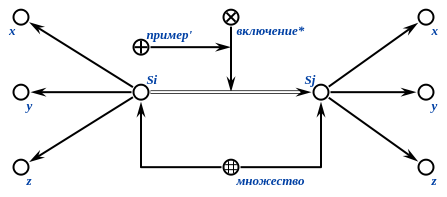
\includegraphics[scale=0.8]{images/part2/chapter_top_ontologies/inclusion.png}
	\label{scg_example_set}
\end{figure}

\begin{comment}
	
\scnheader{множество без кратных элементов}
\scnidtf{классическое множество}
\scnidtf{канторовское множество}
\scnidtf{множество, состоящее из разных элементов}
\scnidtf{множество без кратного вхождения элементов}
\scnidtf{множество, все элементы которого входят в него однократно}
\scnidtf{множество, не имеющее кратного вхождения элементов}
\scnexplanation{\textbf{\textit{множество без кратных элементов}} - это \textit{множество}, для каждого элемента которого существует только одна пара принадлежности, выходящая из знака этого множества в указанный элемент.}

\scnheader{нечеткое множество}
\scnexplanation{\textbf{\textit{нечеткое множество}} --- это \textit{множество}, которое представляет собой совокупность элементов произвольной природы, относительно которых нельзя точно утверждать --- обладают ли эти элементы некоторым характеристическим свойством, которое используется для задания этого нечеткого множества. Принадлежность элементов такому множеству указывается при помощи \textit{нечетких позитивных sc-дуг принадлежности}.}

\scnheader{четкое множество}
\scnexplanation{\textbf{\textit{четкое множество}} --- это \textit{множество}, принадлежность элементов которому достоверна и указывается при помощи \textit{четких позитивных sc-дуг принадлежности}.}

\scnheader{мультимножество}
\scnidtf{множество, имеющее кратные вхождения хотя бы одного элемента}
\scnidtf{множество, по крайней мере один элемент которого входит в его состав многократно}
\scnexplanation{\textbf{\textit{мультимножество}} - это \textit{множество}, для которого существует хотя бы одна кратная пара принадлежности, выходящая из знака этого множества.}

\scnheader{множество первичных сущностей}
\scnsuperset{класс первичных сущностей}
\scnsubset{множество}
\scnexplanation{\textbf{\textit{множество первичных сущностей}} --- это \textit{множество}, элементы которого не являются знаками множеств.}

\scnheader{семейство множеств}
\scnidtf{множество множеств}
\scnsuperset{класс классов}
\scnexplanation{\textbf{\textit{семейство множеств}} --- это \textit{множество}, элементами которого являются знаки множеств.}

\scnheader{нерефлексивное множество}
\scnexplanation{\textbf{\textit{нерефлексивное множеств}} --- это \textit{множество}, знак которого не является элементом этого множества}

\scnheader{рефлексивное множество}
\scnexplanation{\textbf{\textit{рефлексивное множеств}} --- это \textit{множество}, знак которого является элементом этого множества}

\end{SCn}

\begin{SCn}
\scnheader{принадлежность*}
\scnidtf{принадлежность элемента множеству*}
\scnidtf{отношение принадлежности элемента множеству*}
\scniselement{бинарное отношение}
\scniselement{ориентированное отношение}
\end{SCn}

\textbf{\textit{принадлежность*}} --- это \textit{бинарное ориентированное отношение}, каждая связка которого связывает множество с одним из его элементов. Элементами отношения \textit{принадлежность*} по умолчанию являются \textit{позитивные sc-дуги принадлежности}.

\begin{SCn}
\scnheader{класс}
\scnidtf{класс sc-элементов}
\begin{scnrelfromset}{разбиение}
	\scnitem{класс первичных sc-элементов}
	\scnitem{класс множеств}
\end{scnrelfromset}
\end{SCn}

\textbf{\textit{класс}} --- множество элементов, обладающих какими-либо явно указываемыми общими свойствами.

\begin{SCn}
\scnheader{включение*}
\scnidtftext{часто используемый sc-идентификатор}{включает*}
\scnidtftext{часто используемый sc-идентификатор}{включает в себя*}
\scnidtf{включение множеств*}
\scnidtf{быть подмножеством*}
\scniselement{бинарное отношение}
\scniselement{ориентированное отношение}
\scniselement{транзитивное отношение}
\scnrelfrom{область определения}{множество}
\scnsuperset{строгое включение*}
\end{SCn}

\textbf{\textit{включение*}} --- это бинарное ориентированное отношение, каждая связка которого связывает два множества. Будем говорить, что \textit{Множество Si} \textit{включает*} в себя \textit{Множество Sj} в том и только том случае, если каждый элемент \textit{Множества Sj} является также и элементом \textit{Множества Si}

\begin{SCn}
\scnheader{объединение*}
\scnidtf{объединение множеств*}
\scniselement{квазибинарное отношение}
\scniselement{ориентированное отношение}
\end{SCn}

\textbf{\textit{объединение*}} --- это \textit{квазибинарное ориентированное отношение}, областью определения которого является семейство всевозможных множеств. Будем говорить, что \textit{Множество Si} является объединением \textit{Множество Sj} и \textit{Множество Sk} тогда и только тогда, когда любой элемент \textit{Множество Si} является элементом или \textit{Множество Sj} или \textit{Множество Sk}.

\begin{SCn}
\scnheader{разбиение*}
\scnidtf{разбиение множества*}
\scnidtf{объединение попарно непересекающихся множеств*}
\scnidtf{декомпозиция множества*}
\scniselement{квазибинарное отношение}
\scniselement{ориентированное отношение}
\scniselement{отношение декомпозиции}
\end{SCn}
	
\textbf{\textit{разбиение*}} --- это \textit{квазибинарное ориентированное отношение}, областью определения которого является семейство всевозможных множеств. В результате разбиения множества получается множество попарно непересекающихся множеств, объединение которых есть исходное множество.

Семейство множеств \{\textit{S1…, Sn}\} является разбиением множества \textit{Si} в том и только том случае, если:
\begin{textitemize}
	\item семейство \{\textit{S1…, Sn}\} является семейством \textit{попарно непересекающихся множеств};
	\item семейство \{\textit{S1…, Sn}\} является покрытием множества \textit{Si} (или другими словами, множество \textit{Si} является \textit{объединением} множеств, входящих в указанное выше семейство).
\end{textitemize}

\begin{SCn}
\scnheader{пересечение*}
\scnidtf{пересечение множеств*}
\scniselement{квазибинарное отношение}
\scniselement{ориентированное отношение}
\end{SCn}

\textbf{\textit{пересечение*}} --- это операция над множествами, аргументами которой являются два или большее число множеств, а результатом является множество, элементами которого являются все те и только те сущности, которые одновременно принадлежат каждому множеству, которое входит в семейство аргументов этой операции.

Будем говорить, что \textit{Множество Si} является пересечением \textit{Множество Sj} и \textit{Множество Sk} тогда и только тогда, когда любой элемент \textit{Множество Si} является элементом \textit{Множество Sj} и элементом \textit{Множество Sk}.

\begin{SCn}
\scnheader{пара пересекающихся множеств*}
\scniselement{бинарное отношение}
\scniselement{неориентированное отношение}
\scnexplanation{\textbf{\textit{пара пересекающихся множеств*}} --- \textit{бинарное неориентированное отношение} между двумя \textit{множествами}, имеющими непустое \textit{пересечение*}.}
\scntext{определение}{\textit{пара пересекающихся множеств*} --- \textit{бинарное неориентированное отношение} между двумя \textit{множествами}, имеющими, по крайней мере, один общий для этих двух множеств элемент.}
\end{SCn}

\begin{SCn}
\scnheader{попарно пересекающиеся множества*}
\scnidtf{семейство попарно пересекающихся множеств*}
\scnsuperset{пересекающиеся множества*}
\scniselement{отношение}
\scntext{определение}{\textbf{\textit{попарно пересекающиеся множества*}} --- семейство множеств, каждая пара которых является парой пересекающихся множеств, то есть каждая пара которых имеет хотя бы один общий элемент}
\scntext{примечание}{Не каждое \textit{семейство попарно пересекающихся множеств*} является \textit{семейством пересекающихся множеств*}, хотя обратное верно.}
\end{SCn}

\begin{SCn}
\scnheader{декартово произведение*}
\scnidtf{декартово произведение множеств*}
\scnidtf{прямое произведение множеств*}
\scniselement{бинарное отношение}
\scniselement{ориентированное отношение}
\end{SCn}

\textbf{\textit{декартово произведение*}} --- это \textit{бинарное ориентированное отношение} между \textit{ориентированной парой} множеств и \textit{множеством}, элементами которого являются всевозможные упорядоченные пары, первыми элементами которых являются элементы первого из указанных множеств, вторыми --- элементы второго из указанных множеств.


\begin{SCn}
\scnheader{мощность множества}
\scnidtf{кардинальное число}
\scnidtf{общее число вхождений элементов в заданное множество}
\scnidtf{класс эквивалентности, элементами которого являются знаки всех тех и только тех множеств, которые имеют одинаковую мощность}
\scnidtf{класс эквивалентности, соответствующий отношению быть парой множеств, имеющих одинаковую мощность (равномощность множеств)}
\scnidtf{величина мощности множеств}
\scnidtf{трансфинитное число}
\scnidtf{мощность по Кантору}
\scniselement{параметр}
\end{SCn}

\textbf{\textit{мощность множества}} --- это \textit{параметр}, элементами которых являются \textit{множества}, имеющие одинаковое количество элементов. Значением данного параметра является числовая величина, задающая количество элементов, входящих в данный класс множеств, то есть по сути, количество \textit{позитивных sc-дуг принадлежности}, выходящих из данного \textit{множества}.
	
Для двух множеств, имеющих одинаковую мощность, существует взаимно-однозначное соответствие между ними (между множествами вхождений элементов в эти множества --- на случай мультимножеств).
\end{comment}

\section{Формальная онтология связок и отношений}
\label{sec_top_ontologies_rel}

\textit{связь} --- \textit{множество}, являющееся абстрактной моделью связи между описываемыми сущностями, которые или знаки которых являются элементами этого \textit{множества}.

\begin{SCn}
\scnheader{связь}
\begin{scnsubdividing}
	\scnitem{бинарная связь}
	\scnitem{небинарная связь}
\end{scnsubdividing}

\begin{scnsubdividing}
	\scnitem{неориентированная связь}
	\scnitem{ориентированная связь}
\end{scnsubdividing}
\end{SCn}
	
\begin{comment}		
	
\scnheader{бинарная связь}
\begin{scnsubdividing}
	\scnitem{sc-коннектор}
	\scnitem{неатомарная бинарная связь}
\end{scnsubdividing}
\end{SCn}

Данное разбиение осуществляется на основе синтаксического признака, а не семантического, поскольку каждый \textit{sc-коннектор} может быть записан в памяти при помощи семантически эквивалентной конструкции, содержащей знак самой связи и пары принадлежности, ведущие к ее элементам, уточненные, при необходимости ролевыми отношениями.

Каждый \textbf{\textit{sc-коннектор}} представлен в \textit{sc-памяти} одним \textit{sc-элементом} и семантически эквивалентен конструкции, содержащей знак некоторой \textit{бинарной связи} и пары принадлежности, ведущие к элементам этой связи, уточненные, при необходимости ролевыми отношениями.

Такая конструкция может быть обозначена \textbf{\textit{sc-коннектором}} только в случае, когда роли компонентов соответствующей бинарной связи указываются только при помощи \textit{числовых атрибутов 1\scnrolesign} и \textit{2\scnrolesign} или не уточняются вообще.
	
\textbf{\textit{небинарная связь}} --- \textit{связь}, имеющая больше двух элементов.

\begin{SCn}
	
	\scnheader{неориентированная связь}
	\scnsuperset{неориентированное множество}
	\scnexplanation{\textbf{\textit{неориентированная связь}} --- связь, все элементы которой имеют одинаковые роли (при этом соответствующее ролевое отношение, как правило, явно не указывается).}
	
	\scnheader{ориентированная связь}
	\scnsuperset{кортеж}
	\scnexplanation{\textbf{\textit{ориентированная связь}} --- связь, в которой с помощью ролевых отношений, указываются роли компонентов этой связи.}
	
	\scnheader{отношение}
	\scnidtf{класс связей}
	\scnidtf{класс sc-связок}
	\scnidtf{множество отношений}
	\scnidtf{Множество всевозможных отношений}
	\scntext{определение}{\textbf{\textit{отношение}}, \textit{заданное на множестве M} --- это подмножество \textit{декартового произведения} этого множества самого на себя некоторое количество раз}
\end{SCn}
\end{comment}
\textbf{\textit{отношение}}, \textit{заданное на множестве M} --- это подмножество \textit{декартового произведения} этого множества самого на себя некоторое количество раз. В более широком смысле \textbf{\textit{отношение}} --- это математическая структура, которая формально определяет свойства различных объектов и их взаимосвязи.

\begin{SCn}
\scnheader{отношение}
\begin{scnsubdividing}
	\scnitem{класс равномощных связок}
	\scnitem{класс связок разной мощности}
\end{scnsubdividing}
\begin{scnsubdividing}
	\scnitem{бинарное отношение}
	\scnitem{небинарное отношение}
\end{scnsubdividing}
\begin{scnsubdividing}
	\scnitem{ориентированное отношение}
	\scnitem{неориентированное отношение}
\end{scnsubdividing}
\begin{scnsubdividing}
	\scnitem{ролевое отношение}
	\scnitem{неролевое отношение}
\end{scnsubdividing}
	
\scnheader{бинарное отношение}
\scnsuperset{квазибинарное отношение}
\scnsuperset{отношение порядка}
\scnsuperset{отношение толерантности}
\begin{scnsubdividing}
	\scnitem{рефлексивное отношение}
	\scnitem{антирефлексивное отношение}
	\scnitem{частично рефлексивное отношение}
\end{scnsubdividing}
\begin{scnsubdividing}
	\scnitem{симметричное отношение}
	\scnitem{антисимметричное отношение}
	\scnitem{частично симметричное отношение}
\end{scnsubdividing}
\begin{scnsubdividing}
	\scnitem{транзитивное отношение}
	\scnitem{антитранзитивное отношение}
	\scnitem{частично транзитивное отношение}
\end{scnsubdividing}
\begin{scnsubdividing}
	\scnitem{ролевое отношение}
	\scnitem{неролевое бинарное отношение}
\end{scnsubdividing}
\end{SCn}


На \textit{\nameref{scg_example_side_relation}} приведён пример отношения сторона*.

\begin{figure}
	\centering
	\caption{Рисунок. Пример формализации отношения}
	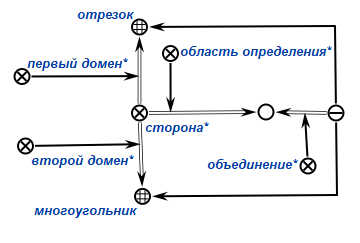
\includegraphics[scale=0.8]{images/part2/chapter_top_ontologies/union_relation.png}
	\label{scg_example_side_relation}
\end{figure}

\begin{comment}
	

Если \textit{бинарное отношение R} задано на \textit{множестве} \textit{\textit{М}} и два элемента этого множества \textit{\textit{a}} и \textit{\textit{b}} связаны данным отношением, то будем обозначать такую связь как \textit{\textit{aRb}}.
	
\begin{SCn}
\scnheader{квазибинарное отношение}
\scnexplanation{\textbf{\textit{квазибинарное отношение}} --- \textit{множество ориентированных пар}, первые компоненты которых являются связками.}
\end{SCn}

Таким образом, \textit{sc-дуги}, принадлежащие \textit{\textit{квазибинарным отношениям}}, всегда выходят из связок.

\begin{SCn}
\scntext{sc-утверждение}{В область определения квазибинарного отношения будем включать:
\begin{scnitemize}
	\item вторые компоненты ориентированных пар, принадлежащих этому отношению;
	\item элементы первых компонентов ориентированных пар, принадлежащих этому отношению;
	\item других элементов область определения квазибинарного отношения не содержит.
\end{scnitemize}
}
	
\scnheader{связанное отношение*}
\scniselement{бинарное отношение}
\scntext{определение}{\textbf{\textit{связанное отношение* R}} на \textit{множестве} \textit{\textit{A}} --- это \textit{бинарное отношение}, в котором для каждой пары элементов \textit{\textit{а}} и \textit{\textit{b}} этого множества выполняется одно из двух отношений: \textit{\textit{aRb}} или \textit{\textit{bRa}}.}
	
\scnheader{отношение порядка}
\begin{scnsubdividing}
	\scnitem{отношение строгого порядка}
	\scnitem{отношение нестрогого порядка}
\end{scnsubdividing}
	
\scntext{определение}{\textbf{\textit{отношение порядка}} --- это \textit{бинарное отношение}, обладающее свойством транзитивности и антисимметричности.}
\end{SCn}

\scnheader{отношение строгого порядка}
\scntext{определение}{\textbf{\textit{отношение строгого порядка}} --- это \textit{отношение порядка}, обладающее свойством антирефлексивности.}
	
\scnheader{отношение нестрогого порядка}
\scntext{определение}{\textbf{\textit{отношение нестрогого порядка}} --- это \textit{отношение порядка}, обладающее свойством рефлексивности.}
	
\scnheader{отношение толерантности}
\scntext{определение}{\textbf{\textit{отношение толерантности}} --- это \textit{бинарное отношение}, принадлежащее классам \textit{симметричное отношение} и \textit{рефлексивное отношение}.}
	
\scnheader{отношение эквивалентности}
\scnidtf{максимальное семейство отношений эквивалентности}
\scnsubset{отношение толерантности}
\scntext{определение}{\textbf{\textit{отношение эквивалентности}} --- это \textit{отношение толерантности}, принадлежащее классу \textit{транзитивных отношений}}
\scntext{примечание}{Каждое отношение эквивалентности уточняет то, что мы считаем эквивалентными сущностями, то есть то, на какие сходства этих сущностей мы обращаем внимание и какие их отличия мы игнорируем (не учитываем).}
	
\scnheader{ролевое отношение}
\scnidtf{атрибут}
\scnidtf{атрибутивное отношение}
\scnidtf{отношение, которое задает роль элементов в рамках некоторого множества}
\scnidtf{отношение, являющееся подмножеством отношения принадлежности}
\scnrelto{семейство подмножеств}{принадлежность*}
\scnsubset{бинарное отношение}
\scnsuperset{числовой атрибут}
\scnexplanation{\textbf{\textit{ролевое отношение}} --- это отношение, являющееся подмножеством отношения принадлежности.}
\scntext{правило идентификации экземпляров}{В конце каждого \textit{идентификатора}, соответствующего экземплярам класса \textbf{\textit{ролевое отношение}}, не являющегося системным, ставится знак ``\scnrolesign''.
	
Например:\\
\textit{ключевой экземпляр\scnrolesign}
	
Из-за ограничений в разрешенном алфавите символов, в системном идентификаторе не может быть использовать знак ``\scnrolesign'', поэтому в начале каждого \textit{системного идентификатора}, соответствующего экземплярам класса \textbf{\textit{ролевое отношение}} ставится префикс ``rrel\_''.
	
Например:\\
\textit{rrel\_key\_sc\_element}}
	
\scnheader{числовой атрибут}
\scnidtf{порядковый номер}
\scnidtf{номер компонента ориентированной связки}
\scnhaselement{\textit{1\scnrolesign}}
\scnhaselement{\textit{2\scnrolesign}}
\scnhaselement{\textit{3\scnrolesign}}
\scnexplanation{\textbf{\textit{числовой атрибут}} --- \textit{ролевое отношение}, задающее порядковый номер элемента некоторой ориентированной связки, не уточняя при этом семантику такой принадлежности. Во многих случаях бывает достаточно использовать числовые атрибуты, чтобы различать компоненты связки, семантика каждого из которых дополнительно оговаривается, например, при определении отношения, которому данная связка принадлежит.}
	
\scnheader{неролевое отношение}
\begin{scnsubdividing}
	\scnitem{небинарное отношение}
	\scnitem{неролевое бинарное отношение}
\end{scnsubdividing}
\scnexplanation{\textbf{\textit{неролевое отношение}} --- отношение, не являющееся подмножеством отношения принадлежности.}
\scntext{правило идентификации экземпляров}{В конце каждого \textit{идентификатора}, соответствующего экземплярам класса \textbf{\textit{неролевое отношение}}, не являющегося системным, ставится знак ``*''.
	
Например:\\
\textit{включение*}
	
Из-за ограничений в разрешенном алфавите символов, в системном идентификаторе не может быть использовать знак ``*'', поэтому в начале каждого \textit{системного идентификатора}, соответствующего экземплярам класса \textbf{\textit{неролевое отношение}} ставится префикс ``nrel\_''.
	
Например:\\
\textit{nrel\_inclusion}}
	
	
\scnheader{арность}
\scnidtf{арность отношения}
\scniselement{параметр}
\scnexplanation{\textbf{\textit{арность}} --- это параметр, каждый элемент которого представляет собой класс \textit{отношений}, каждая связка которых имеет одинаковую \textit{мощность}. Значение данного \textit{параметра} совпадает со значением \textit{мощности} каждой из таких связок.}
	
\scnheader{область определения*}
\scnidtf{область определения отношения*}
\scniselement{бинарное отношение}
\scnexplanation{\textbf{\textit{область определения*}} --- это \textit{бинарное отношение}, связывающее отношение со множеством, являющимся его областью определения.
	
Областью определения отношения будем называть результат теоретико-множественного объединения всех связок этого отношения, или, другими словами, результат теоретико-множественного объединения всех множеств, являющихся доменами данного отношения.}
	
\scnheader{атрибут отношения*}
\scnidtf{ролевой атрибут, используемый в связках заданного отношения*}
\scniselement{бинарное отношение}
\scnexplanation{\textbf{\textit{атрибут отношения*}} --- это \textit{бинарное отношение}, связывающее заданное отношение с \textit{ролевым отношением}, используемым в данном отношении для уточнения роли того или иного элемента связок данного отношения.}
	
\scnheader{домен*}
\scnidtf{домен отношения по заданному атрибуту*}
\scniselement{бинарное отношение}
\scnexplanation{\textbf{\textit{домен*}} --- это \textit{бинарное отношение}, связывающее связку отношения \textit{атрибут отношения*} со множеством, являющимся доменом заданного отношения по заданному атрибуту. Множество \textit{\textit{di}} является доменом отношения \textit{\textit{ri}} по атрибуту \textit{\textit{ai}} в том и только том случае, если элементами этого множества являются все те и только те элементы связок отношения \textit{\textit{ri}}, которые имеют в рамках этих связок атрибут \textit{\textit{ai}}.}
	
\scnheader{соответствие*}
\scnidtf{наличие соответствия*}
\scniselement{бинарное отношение}
\begin{scnsubdividing}
	\scnitem{соответствие между непересекающимися множествами*}
	\scnitem{соответствие между строго пересекающимися множествами*}
	\scnitem{соответствие, область отправления и область прибытия которого совпадают*}
\end{scnsubdividing}
\begin{scnsubdividing}
	\scnitem{всюду определенное соответствие*}
	\scnitem{частично определенное соответствие*}
\end{scnsubdividing}
\begin{scnsubdividing}
	\scnitem{сюръекция*}
	\scnitem{несюръективное соответствие*}
\end{scnsubdividing}
\begin{scnsubdividing}
	\scnitem{однозначное соответствие*}
	\scnitem{неоднозначное соответствие*}
\end{scnsubdividing}
\scntext{определение}{\textbf{\textit{соответствие*}} --- \textit{бинарное ориентированное отношение}, каждая пара которого связывает два множества и указывает на наличие некоторого отношения, связывающего элементы этих двух множеств.}
	
	
\scnheader{область отправления\scnrolesign}
\scnidtf{область отправления соответствия\scnrolesign}
\scnidtf{область определения соответствия\scnrolesign}
\scnidtf{первый компонент пары в отношении соответствия\scnrolesign}
\scniselement{ролевое отношение}
\scntext{определение}{\textbf{\textit{область отправления\scnrolesign}} --- \textit{ролевое отношение}, указывающее на первый компонент пары в рамках отношения \textit{соответствие*}.}
	
\scnheader{область прибытия\scnrolesign}
\scnidtf{область прибытия соответствия\scnrolesign}
\scnidtf{область значений соответствия\scnrolesign}
\scniselement{ролевое отношение}
\scntext{определение}{\textbf{\textit{область прибытия\scnrolesign}} --- \textit{ролевое отношение}, указывающее на второй компонент пары в рамках отношения \textit{соответствие*}.}
\end{SCn}


\end{comment}
\section{Формальная онтология параметров, величин и шкал}
\label{sec_top_ontologies_params}

Каждый \textbf{\textit{параметр}} представляет собой класс, являющийся семейством всевозможных классов эквивалентности или толерантности, задаваемых либо \textit{отношением эквивалентности}, либо \textit{отношением толерантности} (симметричным, рефлексивным, но частично транзитивным).

Так, например, элементами (значениями, величинами) \textit{параметра} \textit{длина} являются либо классы эквивалентности, задаваемые отношением эквивалентности ``иметь точно одинаковую длину*'', либо классы толерантности, задаваемые отношением вида ``иметь приблизительно одинаковую длину с указываемой точностью*'', либо интервальные классы, задаваемые бинарными отношениями вида ``иметь длину, находящуюся в одном и том же указываемом интервале*'' (например, от 1 метра до 2 метров).

Примерами параметров как отношений эквивалентности являются:

\begin{textitemize}
	\item равновеликость геометрических фигур (по длине, площади, объему --- в зависимости от размерности этих фигур);
	\item иметь одинаковый цвет (быть эквивалентными по цвету);
	\item эквивалентность, по вкусу, запаху, твердости и так далее.
\end{textitemize}

Заметим, что среди элементов (значений, величин) параметра могут встречаться пересекающиеся множества (классы), но объединение всех элементов каждого параметра есть не что иное, как класс всевозможных сущностей, обладающих этим параметром (свойством, характеристикой). Например, класс всех сущностей, имеющих длину, класс всех сущностей, обладающих цветом.

\begin{SCn}
\scnheader{параметр}
\scnidtf{свойство}
\begin{scnsubdividing}
	\scnitem{измеряемый параметр}
	\scnitem{неизмеряемый параметр}
\end{scnsubdividing}
\end{SCn}
		
		
На \textit{\nameref{scg_example_parameter}} приведён пример неизмеряемого параметра "цвет" и измеряемых параметров "длина" и "масса".

\begin{figure}
	\centering
	\caption{Рисунок. Пример формализации параметра}
	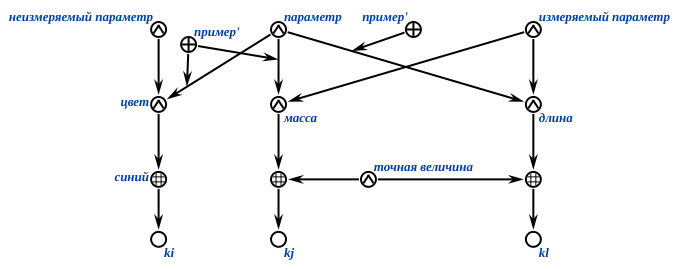
\includegraphics[scale=0.8]{images/part2/chapter_top_ontologies/parameterDescription.png}
	\label{scg_example_parameter}
\end{figure}

Каждый конкретный параметр (характеристика), то есть каждый элемент класса всевозможных параметров (характеристик) есть, по сути, признак классификации сущностей, обладающих это характеристикой, по принципу эквивалентности (одинаковости значения) этой характеристики. Например, параметр \textit{цвет} разбивает множество сущностей имеющих цвет на классы, каждый из которых включает в себя сущности, имеющие одинаковый цвет.
		
Другими словами, каждому множеству сущностей может ставиться в соответствие набор (семейство) параметров (параметрическое пространство), которыми обладают сущности этого множества --- аналог семейства отношений, определенных (заданных) на этом множестве. Часто бывает важно построить такое параметрическое пространство, "точки"{} которого взаимнооднозначно соответствуют параметризуемым сущностям (например, набор параметров, позволяющих однозначно идентифицировать, установить личность каждого человека). 


\begin{comment}
\begin{SCn}
\scnheader{область определения параметра*}
\scnidtf{множество всех тех и только тех сущностей, которые являются компонентами значений заданного параметра*}
\scnidtf{множество всех тех и только тех сущностей, которые обладают заданным параметром*}
\scnrelto{включение}{объединение*}

\bigskip
\scnheader{измеряемый параметр}
\scnidtf{количественный параметр}
\scnidtf{семейство измеряемых величин}
\scnidtf{семейство классов эквивалентности, каждому из которых может быть поставлено в соответствие числовое значение}
\end{SCn}

Каждый \textbf{\textit{измеряемый параметр}} представляет собой \textit{параметр}, значение (элемент, экземпляр) которого трактуется как \textit{величина}, которой можно поставить в соответствие ее числовое значение на основании выбранной единицы измерения и/или точки отсчета (нулевой отметки выбранной шкалы).

\begin{SCn}
\scnsuperset{параметр, измеряемый по шкале}
	
\scnheader{неизмеряемый параметр}
\scnidtf{качественный параметр}
	
\scnheader{ориентированный параметр}
\scnidtf{упорядоченный параметр}
\scnsuperset{параметр, измеряемый по шкале}
\scnidtf{параметр, на значениях которого может быть задано некоторое отношение порядка, семантика которого уточняется в зависимости от семантики параметра}
	

\scnheader{величина}
\scnidtf{значение количественного параметра}
\scnidtf{значение измеряемого параметра}
\scnidtf{класс сущностей, имеющих одинаковое значение соответствующего параметра}
\begin{scnrelfromlist}{включение}
	\scnitem{точная величина}
	\scnitem{неточная величина}
	\scnitem{интервальная величина}
\end{scnrelfromlist}
\end{SCn}

Каждая \textbf{\textit{величина}} представляет собой однозначный и независящий от шкалы измерения результат измерения некоторой характеристики у некоторой сущности.
		
Каждой \textit{величине} можно поставить в соответствие ее числовое значение на основании выбранной единицы измерения и точки отсчета (нулевой отметки выбранной шкалы, в случае, если измерение осуществляется по шкале).
		
Нельзя путать значение параметра (\textit{величину}) и значение величины по некоторой шкале, которое может быть скалярным и векторным.
	
\begin{SCn}
\scnheader{точная величина}
\scnidtf{точное значение параметра}
\scnidtf{множество всех точных значений параметра}
\scnidtf{значение параметра, являющееся семейством классов эквивалентности, соответствующим некоторому отношению эквивалентности}
\scnidtf{класс эквивалентности}
\end{SCn}

Каждая \textbf{\textit{точная величина}} имеет одно фиксированное значение в некоторой единице измерения или по какой-либо шкале. При этом считается, что все элементы такого класса имеют одинаковое значение данного параметра и отклонениями можно пренебречь.
		
Каждой \textit{точной величине} можно поставить в соответствие группу \textit{неточных величин}, являющихся не разбиениями, а покрытиями того же множества, но с разной степенью точности.

\begin{SCn}
\scnheader{неточная величина}
\scnidtf{множество неточных значений параметра}
\scnidtf{приблизительная величина}
\scnidtf{приблизительное значение параметра}
\scnidtf{значение параметра в интервале с нефиксированными границами}
\end{SCn}

Каждой \textbf{\textit{неточной величине}} ставится в соответствие ее значение в некоторой единице измерения или по какой-либо шкале, а также дополнительно указывается \textit{точность*}, то есть возможное отклонение от данного значения.

\begin{SCn}
\scnheader{интервальная  величина}
\scnidtf{интервальное значение параметра}
\scnidtf{значение параметра в интервале с фиксированными границами}
\scnidtf{интервал значения параметра из множества пересекающихся интервалов разной длины, имеющих нефиксированные границы}
\end{SCn}

Каждая \textbf{\textit{интервальная величина}} представляет собой класс сущностей, находящихся в рамках точно заданного интервала, минимальная и максимальная точка которого являются \textit{точными величинами}. Результатом \textit{измерения*} такой величины является ориентированная пара, первым компонентом которой является левая (меньшая) граница интервала, вторым компонентом --- правая (большая) граница интервала.

\begin{SCn}
\scnheader{эталон\scnrolesign}
\scnidtf{образец\scnrolesign}
\scniselement{ролевое отношение}
\end{SCn}

\begin{SCn}
Ролевое отношение \textit{эталон\scnrolesign} указывает на тот элемент значения некоторого параметра, который в рамках данного класса эквивалентности считается эталонным, то есть он используется как образец при определении данного параметра.
\end{SCn}
		
\begin{SCn}
\textit{эталон\scnrolesign} может задаваться как для измеряемых, так и для неизмеряемых параметров, например, эталон метра или эталон красоты.
\end{SCn}
	
\begin{SCn}
\scnheader{измерение*}
\scnidtf{значение параметра*}
\scnidtf{значение заданной величины заданного параметра*}
\scnidtf{измерение как соответствие*}
\scnidtf{результат измерения заданной величины в заданной единице измерения и по заданной шкале*}
\scnidtf{бинарное ориентированное отношение, связывающее различные величины с результатами их измерения в различных единицах измерения и по различным шкалам*}
\end{SCn}

Связки отношения \textit{измерение*} связывают величину и ее значение в некоторой единице измерения (в том числе, в интервале) или по некоторой шкале. Конкретная единица измерения или шкала указывается дополнительно при помощи соответствующего отношения. Одной величине может соответствовать только одно значение в каждой возможной единице измерения или одна точка на некоторой шкале.
	
	
\begin{SCn}
\scnheader{единица измерения*}
\scniselement{бинарное отношение}
\scnidtf{единица по шкале*}
\scnidtf{единичная отметка по шкале*}
\end{SCn}

Связки отношения \textbf{\textit{единица измерения*}} связывают знак конкретного \textbf{\textit{измерения с фиксированной единицей измерения}} и некоторую \textit{точную величину}, входящую в тот же конкретный \textit{параметр}, что и первый компонент связок этого конкретного измерения, и которая используется в данном случае в качестве единицы измерения.
	
\begin{SCn}
\scnheader{измерение по шкале}
\scnidtf{шкала}
\scnrelto{семейство подмножеств}{измерение*}
\end{SCn}

Каждая \textbf{\textit{измерение по шкале}} представляет собой подмножество отношения \textit{измерение*} и характеризуется не единицей измерения, а некоторой точкой отсчета для данной \textbf{\textit{шкалы}}. Результатом \textit{измерения по шкале} будет некоторая точка шкалы, отстоящая от точки отсчета на определенное расстояние в нужную сторону (меньшую или большую). Понятно, что это расстояние может быть измерено любыми единицами измерения, но его величина при этом останется неизменной.
		
Не стоит путать измерение по \textit{измерение по шкале}, которое зависит от \textit{нулевой отметки*}, с измерением изменения того же \textit{параметра}, которое характеризуется единицей измерения и не зависит от точки отсчета. Например, не стоит путать дату по некоторому календарю, соответствующую \textit{началу} какого-либо процесса, и \textit{длительность} этого процесса, которая не зависит от выбранного календаря.

Каждое \textbf{\textit{арифметическое выражение на величинах}} представляет собой \textit{связку}, компонентами которой являются элементы или подмножества некоторого \textit{количественного параметра}.

\bigskip
\bigskip
\bigskip
\bigskip
\begin{SCn}
\scnheader{действие. измерение}
\scnidtf{измерение как действие}
\scnidtf{действие, направленное на установление связи, принадлежащей отношению измерение* и связывающей величину, которая принадлежит заданному параметру, и которой принадлежит заданная сущность, и соответствующее значение этой величины на некоторой шкале}
\scnidtf{действие, направленное на решение задачи измерения заданного параметра у заданной сущности}
\scnrelto{включение}{действие}
	
\scnheader{задача. измерение}
\scnidtf{спецификация действия измерения}
\scnidtf{спецификация действия, целью которого является измерение заданного параметра у заданной сущности}
\scnrelto{включение}{задача}
\end{SCn}	
\end{comment}

\begin{comment}
	

\section{Формальная онтология чисел и числовых структур}
\label{sec_top_ontologies_numbers}
	
\begin{SCn}
\begin{scnrelfromlist}{ключевое понятие}
	\scnitem{число}
	\scnitem{цифра}
\end{scnrelfromlist}

\begin{scnrelfromlist}{ключевое отношение}
	\scnitem{модуль*}
	\scnitem{арифметическая операция*}
	\scnitem{произведение*}
\end{scnrelfromlist}
\end{SCn}

\textbf{\textit{число}} --- это основное понятие математики, используемое для количественной характеристики, сравнения, нумерации объектов и их частей. Письменными знаками для обозначения чисел служат \textit{цифры}.

\begin{SCn}
\scnheader{цифра}
\scnidtf{множество цифр}
\scnsubset{внутренний файл ostis-системы}
\begin{scnrelfromlist}{включение}
	\scnitem{арабская цифра}
	\scnitem{римская цифра}
\end{scnrelfromlist}
\end{SCn}

\textbf{\textit{цифра}} --- это множество файлов, обозначающих вхождение этой цифры во всевозможные записи чисел с помощью этой цифры.

\begin{SCn}
\scnheader{натуральное число}
\scnidtf{множество натуральных чисел}
\scnsubset{целое число}
\end{SCn}

\textbf{\textit{натуральное число}} --- это подмножество множества \textit{целых чисел}, которые используются при счете предметов.


\begin{SCn}
\scnheader{рациональное число}
\scnidtf{множество рациональных чисел}
\scnsubset{действительное число}
\scnsubset{целое число}
\end{SCn}

\textbf{\textit{рациональное число}} --- это число, представляемое \textit{обыкновенной дробью}, где числитель — \textit{целое число}, а знаменатель — \textit{натуральное число}.

\begin{SCn}
\scnheader{дробь}
\scnidtf{множество дробей}
\begin{scnrelfromlist}{включение}
	\scnitem{обыкновенная дробь}
	\scnitem{десятичная дробь}
\end{scnrelfromlist}
\end{SCn}

\textbf{\textit{дробь}} — это число, состоящее из одной или нескольких равных частей (долей) единицы

\begin{SCn}
\scnheader{обыкновення дробь}
\scnidtf{множество обыкновенных дробей}
\scnidtf{множество простых дробей}
\end{SCn}

\textbf{\textit{обыкновенная дробь}} - запись \textit{рационального числа} в виде ${\displaystyle \pm {\frac {m}{n}}}$ или ${\pm m/n}$, где ${n\neq 0}$.Горизонтальная или косая черта обозначает знак деления, в результате которого получается частное. Делимое называется числителем дроби, а делитель — знаменателем.

\begin{SCn}
\scnheader{десятичная дробь}
\scnidtf{множество десятичных дробей}
\end{SCn}

\textbf{\textit{десятичная дробь}} — разновидность дроби, которая представляет собой способ представления действительных чисел в виде ${\pm d_m \ldots d_1 d_0{,} d_{-1} d_{-2} \ldots}$, где , — десятичная запятая, служащая разделителем между целой и дробной частью числа, ${d_{k}}$m — десятичные цифры.

\begin{SCn}
\scnheader{иррациональное число}
\scnidtf{множество иррациональных чисел}
\scnsubset{действительное число}
\end{SCn}

\textbf{\textit{иррациональное число}} --- это \textit{вещественное число}, которое не является рациональным, то есть не может быть представлено в виде дроби, где числитель — \textit{целое число}, знаменатель — \textit{натуральное число}. Любое \textit{иррациональное число} может быть представлено в виде бесконечной непериодической десятичной дроби.

\begin{SCn}
\scnheader{модуль*}
\scnidtf{модуль числа*}
\scniselement{бинарное отношение}
\scnexplanation{Связки отношения \textbf{\textit{модуль*}} связывают некоторое \textit{число} (которое может быть как \textit{отрицательным}, так и \textit{положительным}) и другое \textit{число} (всегда \textit{положительное}), которое выражает расстояние от указанного числа до \textit{Нуля} в единицах.}
\end{SCn}

\begin{SCn}
\scnheader{арифметическая операция*}
\scnidtf{множество арифметических операций}
\scnrelto{семейство подмножеств}{арифметическое выражение}
\end{SCn}

Каждая \textbf{\textit{арифметическая операция*}} представляет собой \textit{отношение}, элементами которого являются \textit{арифметические выражения}, то есть множество \textit{арифметических выражений} какого-либо одного вида.
	
\begin{SCn}
\scnheader{сумма*}
\scnidtf{сложение*}
\scniselement{арифметическая операция}
\scniselement{квазибинарное отношение}
\end{SCn}

\textbf{\textit{сумма*}} --- это арифметическая операция, в результате которой по данным числам (слагаемым) находится новое число (сумма), обозначающее столько единиц, сколько их содержится во всех слагаемых.
		
Первым компонентом связки отношения \textit{сумма*} является \textit{множество чисел} (слагаемых), содержащее два или более элемента, вторым компонентом --- \textit{число}, являющееся результатом сложения.
		
Отдельно отметим, что каждая связка отношения \textit{сумма*} вида a = b+c может также трактоваться и как запись о вычитании чисел, например b = a-c, в связи с чем \textit{арифметическая операция} разности чисел отдельно не вводится.

\begin{SCn}
\scnheader{произведение*}
\scnidtf{умножение*}
\scniselement{арифметическая операция}
\scniselement{квазибинарное отношение}
\end{SCn}

\textbf{\textit{произведение*}} --- это \textit{арифметическая операция}, в результате которой один аргумент складывается столько раз, сколько показывает другой, затем результат складывается столько раз, сколько показывает третий и так далее.
		
Первым компонентом связки отношения \textit{произведение*} является \textit{множество чисел} (множителей), содержащее два или более элемента, вторым компонентом --- \textit{число}, являющееся результатом произведения.
		
Отдельно отметим, что каждая связка отношения \textit{произведение*} вида a = b*c может также трактоваться и как запись о делении чисел, например b = a/c, в связи с чем \textit{арифметическая операция} деления чисел отдельно не вводится.

\begin{SCn}
\scnheader{возведение в степень*}
\scniselement{арифметическая операция}
\scniselement{бинарное отношение}
\end{SCn}

\textbf{\textit{возведение в степень*}} --- это \textit{арифметическая операция}, в результате которой число, называемое основанием степени, умножается само на себя столько раз, каков показатель степени.
	
Первым компонентом связки отношения \textit{возведение в степень*} является ориентированная пара, первым компонентом которой является \textit{число}, которое является основанием степени, вторым --- \textit{число}, которое является показателем степени; Вторым компонентом связки отношения \textit{возведение в степень*} является \textit{число}, которое является результатом возведения в степень.

\begin{SCn}	
\scnheader{больше*}
\scniselement{бинарное отношение}
\scniselement{отношение строгого порядка}
\scnexplanation{\textbf{\textit{больше*}} --- это \textit{бинарное отношение} сравнения чисел. Из двух чисел на координатной прямой больше то, которое расположено правее. Соответственно, первым компонентом связки \textit{отношения} \textit{больше*} является большее из двух \textit{чисел}.}
\end{SCn}
\end{comment}

\section{Формальная онтология темпоральных сущностей}
\label{sec_top_ontologies_temp}
		
\begin{SCn}
\scnheader{временная сущность}
\scnidtf{сущность, обладающая темпоральными характеристиками (длительностью, начальным моментом, конечным моментом и так далее)}
\begin{scnsubdividing}
	\scnitem{прошлая сущность}
	\scnitem{настоящая сущность}
	\scnitem{будущая сущность}
\end{scnsubdividing}
\begin{scnsubdividing}
	\scnitem{временная связь}
	\scnitem{темпоральная структура}
	\begin{scnindent}
		\scnidtf{структура, содержащая хотя бы одну временную сущность}
		\begin{scnsubdividing}
			\scnitem{ситуация}
			\scnitem{процесс}
		\end{scnsubdividing}
		\end{scnindent}
	\scnitem{материальная сущность}	
\end{scnsubdividing}
\begin{scnsubdividing}
	\scnitem{непрерывная временная сущность}
	\begin{scnindent}
	\begin{scnsubdividing}
		\scnitem{точечная временная сущность}
		\begin{scnindent}
			\scnidtf{временная сущность, длительность существования которой в данном контексте считается несущественной (пренебрежительно малой)}
		\end{scnindent}
		\scnitem{длительная непрерывная временная сущность}
	\end{scnsubdividing}
	\end{scnindent}	
		\scnitem{дискретная временная сущность}
	\begin{scnindent}
		\scnidtf{временная сущность, которая может быть декомпозирована на последовательность точечных временных сущностей}
	\end{scnindent}	
		\scnitem{прерывистая временная сущность}
	\begin{scnindent}
		\scnidtf{временная сущность, являющаяся результатом соединения нескольких не только точечных временных сущностей}
	\end{scnindent}
\end{scnsubdividing}
\end{SCn}	

На \textit{\nameref{scg_example_situation}} приведён пример ситуации. Иванов жил на улице Центральная с 1990 по 1995 год, а затем на улице Весенняя. Здесь указывается начало и конец временного промежутка проживания Иванова на улицах Центральная и Весенняя.

\begin{figure}
	\centering
	\caption{Рисунок. Пример формализации временных сущностей}
	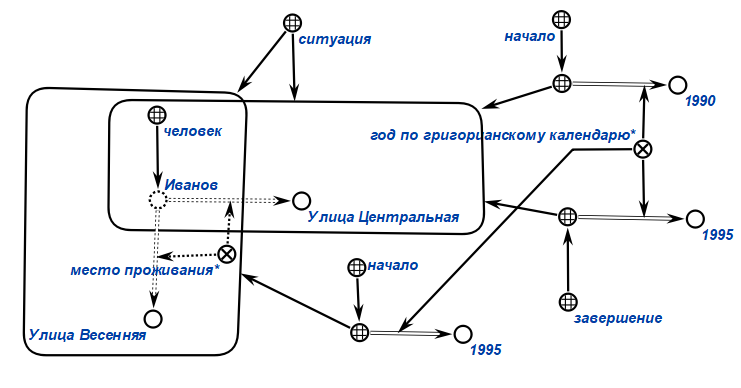
\includegraphics[scale=0.8]{images/part2/chapter_top_ontologies/situation.png}
	\label{scg_example_situation}
\end{figure}

Следует отличать:
	\begin{textitemize}
		\item временный характер сущности, обозначаемой \textit{sc-элементом};
		\item временный характер существования самого \textit{sc-элемента} в рамках \textit{sc-памяти}, поскольку в ходе обработки информации каждый \textit{sc-элемент} может быть удален из \textit{sc-памяти}; 
		\item временный характер описываемых ситуаций, событий и самих процессов;
		\item временный характер хранения в sc-памяти тех sc-конструкций, которые являются самими описаниями соответствующих ситуаций, событий и процессов.
	\end{textitemize}

\begin{comment}
Следует отличать, например, \textit{материальную сущность} (некоторый физический или, в частности, биологический объект) от различных динамических структур (\textit{процессов}), которые с той или иной степенью детализации и в том или ином ракурсе отражают (описывают) динамику изменений этой \textit{материальной сущности}. 
			
При этом сам \textit{процесс} как уточнение динамики некоторой последовательности ситуаций и событий, также является сущностью, принадлежащей к классу \textit{временных сущностей}.


	

\begin{SCn}
\scnheader{прошлая сущность}
\scnidtf{сущность, существовавшая в прошлом времени}
\scnidtf{сущность прошлого времени}
\scnidtf{сущность, завершившая свое существование}

\bigskip
\bigskip
\scnheader{настоящая сущность}
\scnidtf{сущность, существующая в текущий момент времени}
\scnidtf{сущность, существующая сейчас}
\scnidtf{сущность настоящего времени}
		
\scnheader{будущая сущность}
\scnidtf{возможно будущая сущность}
\scnidtf{прогнозируемая временная сущность}
\scnidtf{временная сущность, которая может существовать в будущем}
\scnidtf{сущность, которая может или должна начать свое существование в будущем времени}
\scnrelfrom{включение}{инициированное действие}
\end{SCn}

Каждой \textbf{\textit{будущей сущности}} можно поставить в соответствие вероятность ее возникновения.
	
\begin{SCn}
\scnheader{временная связь}
\scnidtf{нестационарная связь}
\scnidtf{временно существующая связь}
\end{SCn}

Каждая \textbf{\textit{временная связь}} представляет собой \textit{связку}, принадлежащую множеству \textit{временных сущностей}.
			
Понятие \textbf{\textit{временной связи}} не следует путать с понятием \textit{темпоральной связи}, которая сама является \textit{постоянной сущностью}, описывающей то, как связаны во времени некоторые \textit{временные сущности}.

\begin{SCn}
\scnheader{ситуация}
\scnidtf{состояние}
\scnidtf{временная структура}
\scnidtf{временно существующая структура}
\scnidtf{квазистационарная структура}
\scnidtf{состояние некоторой динамической системы, описываемое с некоторой степенью детализации (подробности)}
\scnidtf{квазистационарная структура, существующая временно (в течение некоторого отрезка времени)}
\end{SCn}

Под ситуацией понимается \textit{структура}, содержащая, по крайней мере, один элемент, который является \textit{временной сущностью}. Наличие в рамках ситуации нескольких \textit{временных сущностей} говорит о том, что существует момент времени (в прошлом, настоящем или будущем), в который все они существуют одновременно.

\begin{SCn}
\scnheader{процесс}
\scnidtf{процесс преобразования некоторой временной сущности из одного состояния в другое}
\scnidtf{процесс перехода от одной ситуации к другой}
\scnidtf{абстрактный процесс}
\scnidtf{информационная модель некоторых преобразований}
\scnidtf{динамическая sc-модель}
\scnidtf{динамическая структура}
\scnrelfrom{включение}{воздействие}
\end{SCn}

Каждый \textbf{\textit{процесс}} определяется (задается) либо возникновением или исчезновением связей, связывающих заданную \textit{временную сущность} с другими сущностями, либо возникновением или исчезновением связей, связывающих части указанной \textit{временной сущности} с другими сущностями. 
			
Многим \textit{процессам} можно поставить в соответствие \textit{ситуацию}, которая является его \textit{начальной ситуацией*} и \textit{ситуацию}, которая является его \textit{конечной ситуацией*}, то есть указать \textit{ситуации}, переход между которыми осуществляется в ходе \textit{процесса}.
			
При этом знаки тех \textit{временных сущностей}, с которыми связаны изменения, описываемые некоторым \textit{процессом}, входят в данный \textit{процесс} как элементы и при необходимости уточняются дополнительными \textit{ролевыми отношениями}.

\begin{SCn}
\begin{scnsubdividing}
	\scnitem{процесс в sc-памяти}
	\scnitem{процесс во внешней среде ostis-системы}
\end{scnsubdividing}
\end{SCn}

Каждой \textbf{\textit{материальной сущности}} можно поставить в соответствие различные \textit{процессы}, описывающие ее преобразование из одного состояния в другое.

Поскольку \textit{процесс} представляет собой изменяющуюся во времени динамическую структуру, то полностью представить процесс в базе знаний в общем случае не представляется возможным.
Однако, можно ввести sc-элемент, обозначающий конкретный процесс, с необходимой степенью детализации описать его декомпозицию на более частные подпроцессы и/или описать ситуации, соответствующие состояниям процесса в разные моменты времени.
В данном случае можно провести некоторую аналогию с \textit{бесконечными множествами}, все элементы которых физически не могут быть представлены в базе знаний одновременно, тем не менее, само множество и некоторые из его элементов могут быть описаны с необходимой степенью детализации.
	
\begin{SCn}
\scnheader{воздействие}
\scnidtf{процесс, осуществляющийся на основе (в результате) воздействия одной сущности на другую}
\scnrelfrom{включение}{действие}
\end{SCn}

Каждому \textbf{\textit{воздействию}} может быть поставлена в соответствие (1) некоторая \textit{воздействующая сущность*}, то есть сущность, осуществляющая \textit{воздействие} (в частности, это может быть некоторое физическое поле), и (2) некоторый \textit{объект воздействия*}, то есть сущность, на которую воздействие направлено. Если \textit{воздействие} связано с \textit{материальной сущностью}, то его объектом воздействия является либо сама эта \textit{материальная сущность}, либо некоторая ее пространственная часть.


\begin{SCn}
\scnheader{точечный процесс}
\scnidtf{атомарный процесс}
\scnidtf{условно мгновенный процесс}
\scnidtf{процесс, длительность которого в данном контексте считается несущественной (пренебрежимо малой)}
\scnsubset{точечная временная сущность}
		
\scnheader{элементарный процесс}
\scnidtf{процесс, детализация которого на входящие в него подпроцессы в текущем контексте не производится}
\scnsuperset{точечный процесс}
\end{SCn}

Элементарные процессы могут иметь длительность и, следовательно, не обязательно являются атомарными процессами.

Понятия \textit{точечного процесса} и \textit{элементарного процесса}, как и понятие \textit{точечной временной сущности} в целом, характеризуют не столько характеристики самого \textit{процесса}, сколько степень наших знаний о нем и степень детализации описания процесса в базе знаний. Так, очевидно, что любой процесс, протекающий в компьютерной системе, может быть при необходимости детализирован до уровня команд процессора, затем до уровня микропрограмм и даже до уровня физических процессов (изменения физических характеристик сигналов), однако чаще всего такая детализация не требуется.

\begin{SCn}
\scnheader{событие}
\scnsubset{точечная временная сущность}
\scnidtf{точечная временная сущность, являющаяся началом и/или завершением какой-либо временной сущности (например, процесса)}
\scnidtf{граничная точка временной сущности}

\scnheader{детализация процесса*}
\scnidtf{бинарное ориентированное отношение, каждая связка которого связывает некоторый процесс с более детальным его описанием, что предполагает представление декомпозиции этого процесса на систему взаимосвязанных его подпроцессов (в том числе элементарных).}
\scnrelfrom{пример}{Переход от процесса, соответствующего какой-либо программе, к рассмотрению декомпозиции этого процесса (протокола) в терминах языка программирования высокого уровня, затем переход для каждого из полученных подпроцессов (операторов языка высокого уровня) к детализации выполнения этих подпроцессов на уровне машинных операций, выполняемых процессором компьютера (на уровне ассемблера), и далее к детализации выполнения подпроцессов уровня машинных операций к подпроцессам на уровне языка микропрограммирования. Таким образом, детализация процесса может быть иерархической, вплоть до уровня \textit{элементарных процессов}.}
	\end{comment}
\begin{SCn}
\scnheader{темпоральное отношение}
\scnhaselement{темпоральное включение*}
\scnhaselement{темпоральное объединение*}
\scnhaselement{темпоральная декомпозиция*}
\scnhaselement{темпоральная последовательность*}
\begin{scnindent}
	\begin{scnsubdividing}
	\scnitem{темпоральная смежность*}
	\scnitem{темпоральная последовательность с промежутком*}
	\scnitem{темпоральная последовательность с пересечением*}
	\end{scnsubdividing}
\end{scnindent}
\end{SCn}

\begin{comment}
			
		
\scnheader{темпоральное включение*}
\scnexplanation{Связки отношения \textbf{\textit{темпоральное включение*}} связывают две \textit{временные сущности}, период существования одной из которых полностью включается в период существования второй.\\
Первым компонентом каждой связки отношения \textit{темпоральное включение*} является знак \textit{временной сущности}, \textit{длительность} существования которой больше.}
\scnsuperset{темпоральная часть*}
\scnsuperset{темпоральное включение без совпадения начальных и конечных моментов*}
\scnsuperset{темпоральное совпадение*}
\scnsuperset{темпоральное включение с совпадением начальных моментов*}
\scnsuperset{темпоральное включение с совпадением конечных моментов*}
		
\scnheader{темпоральная часть*}
\scnidtf{этап (период) заданной временной сущности*}
\scnidtf{этап процесса существования временной сущности*}
\scnsuperset{начальный этап*}
\scnsuperset{конечный этап*}
\scnsuperset{промежуточный этап*}
\scnsuperset{подпроцесс*}
\begin{scnindent}
		\scnrelfrom{первый домен}{процесс}
		\scnrelfrom{второй домен}{процесс}
\end{scnindent}
\end{SCn}

Связки отношения \textit{темпоральная часть*} связывают две \textit{временные сущности}, одна из которых является частью другой, например, действие и одно из его поддействий. Соответственно, период существования одной из этих сущностей всегда будет включаться в период существования другой (большей).
			
В отличие от более общего отношения \textit{темпоральное включение*}, связки которого могут связывать любые \textit{временные сущности}, связки отношения \textit{темпоральная часть*} связывают только \textit{временные сущности}, одна из которых является частью другой.

\begin{SCn}
\scnheader{следует отличать*}
\begin{scnhaselementset}
	\scnitem{темпоральная часть*}
	\begin{scnindent}
		\scnsuperset{подпроцесс*}
	\end{scnindent}
	\scnitem{темпоральное включение*}
	\begin{scnindent}
		\scnnote{Связь \textit{темпорального включения*} может связывать абсолютно разные \textit{временные сущности}, существующие в общем случае в разных местах, а не только \textit{временные сущности}, одна из которых является частью другой. Хотя формально и можно объединить любые разные \textit{временные сущности} в одну общую \textit{временную сущность}, далеко не всегда имеет смысл это делать.}
	\end{scnindent}
\end{scnhaselementset}
		
\scnheader{темпоральное включение без совпадения начальных и конечных моментов*}
\scnidtf{строгое темпоральное включение*}
		
\scnheader{начало\scnsupergroupsign}
\scnidtf{одновременность начинаний\scnsupergroupsign}
\scnidtf{класс одновременно начавшихся сущностей\scnsupergroupsign}
\scniselement{параметр}
\end{SCn}

Каждый элемент множества \textbf{начало} представляет собой класс \textit{временных сущностей}, у которых совпадает момент начала их существования. Конкретное значение данного \textit{параметра} может быть как \textit{точной величиной}, так и \textit{неточной величиной} или \textit{интервальной величиной}.


\begin{SCn}
\scnheader{завершение\scnsupergroupsign}
\scnidtf{конец\scnsupergroupsign}
\scnidtf{одновременность завершений\scnsupergroupsign}
\scnidtf{класс одновременно завершившихся сущностей\scnsupergroupsign}
\scniselement{параметр}
\end{SCn}

Каждый элемент множества \textbf{\textit{завершение}} представляет собой класс \textit{временных сущностей}, у которых совпадает конечный момент их существования (момент завершения существования). Конкретное значение данного \textit{параметра} может быть как \textit{точной величиной}, так и \textit{неточной величиной} или \textit{интервальной величиной}.


\begin{SCn}
\scnheader{одновременность\scnsupergroupsign}
\scnidtf{параметр, значениями (элементами) которого являются классы либо одновременно существующих (происходящих) \textit{точечных временных сущностей}, одновременность которых рассматривается с заданной степенью точности, либо одновременно начинающихся и заканчивающихся длительных процессов}
\end{SCn}

Важно отметить, что элементами некоторого значения параметра \textit{одновременности} с заданной точностью могут быть только те временные сущности, которые и начались, и завершились в течение периода времени, заданного указанным значением этого параметра, но при этом начало и завершение этих временных сущностей не обязательно должно совпадать с началом и завершением указанного периода времени. Так, например, можно ввести значение параметра \textit{одновременности} ``\textit{2022 год по Григорианскому календарю}'', элементами которого будут все временные сущности, начавшие и закончившие свое существовавшие в рамках 2022 года. При этом не обязательно, чтобы эти временные сущности начались именно в полночь 1 января 2022 года и закончились в полночь 1 января 2023 года, это могут быть временные сущности, существовавшие, например, в течение июля 2022 года.

\begin{SCn}
\scnheader{следует отличать*}
\begin{scnhaselementset}
\scnitem{темпоральное совпадение*}
	\begin{scnindent}
	\scniselement{отношение эквивалентности}
	\end{scnindent}
	\scnitem{одновременность\scnsupergroupsign}
	\begin{scnindent}
	\scnidtf{фактор-множество для отношения темпоральное совпадение*}
	\end{scnindent}
\end{scnhaselementset}
		
\scnheader{длительность\scnsupergroupsign}
\scnidtf{класс временных сущностей, имеющих одинаковую длительность\scnsupergroupsign}
\scniselement{параметр}
\scnhaselement{тысячелетие}
\scnhaselement{век}
\scnhaselement{год}
\scnhaselement{месяц}
\scnhaselement{день}
\scnhaselement{час}
\scnhaselement{минута}
\scnhaselement{секунда}
\end{SCn}

Каждый элемент множества \textbf{\textit{длительность}} представляет собой класс \textit{временных сущностей}, у которых совпадает длительность их существования. Конкретное значение данного \textit{параметра} может быть как \textit{точной величиной}, так и \textit{неточной величиной} или \textit{интервальной величиной}.
\end{comment}

\begin{comment}

\section{Формальная онтология ситуаций и событий, описывающих динамику баз знаний ostis-систем}
\label{sec_top_ontologies_dynamic}

Обработка информации в \textit{sc-памяти} (то есть динамика базы знаний, хранимой в \textit{sc-памяти}) в конечном счете сводится:
\begin{textitemize}
	\item к появлению в \textit{sc-памяти} новых актуальных \textit{sc-узлов} и \textit{sc-коннекторов};
	\item к логическому удалению актуальных \textit{sc-элементов}, то есть к переводу их в неактуальное состояние (это необходимо для хранения протокола изменения состояния базы знаний, в рамках которого могут описываться действия по удалению \textit{sc-элементов});
	\item к возврату логически удаленных \textit{sс-элементов} в статус актуальных (необходимость в этом может возникнуть при откате базы знаний к какой-нибудь ее прошлой версии);
	\item к физическому удалению \textit{sc-элементов};
	\item к изменению состояния актуальных (логически не удаленных \textit{sc-элементов}) --- \textit{sc-узел} может превратиться в \textit{sc-ребро}, \textit{sc-ребро} может превратиться в \textit{sc-дугу}, \textit{sc-дуга} может поменять направленность, \textit{sc-дуга} общего вида может превратиться в \textit{константную стационарную sc-дугу принадлежности}, и так далее;
\end{textitemize}

Подчеркнем, что временный характер самого \textit{sc-элемента} (так как он может появиться или исчезнуть) никак не связан с возможно временным характером сущности, обозначаемой этим \textit{sc-элементом}. То есть временный характер самого sc-элемента и временный характер сущности, которую он обозначает --- абсолютно разные вещи.

Таким образом, следует четко отличать динамику внешнего мира, описываемого базой знаний, а динамику самой базы знаний (динамику внутреннего мира). При этом очень важно, чтобы описание динамики базы знаний также входило в состав каждой базы знаний.
\end{comment}
\begin{comment}
		

К числу понятий, используемых для описания динамики базы знаний относятся:
\begin{textitemize}
	\item логически удаленный sc-элемент;
	\item сформированное множество;
	\item вычисленное число;
	\item сформированное высказывание;
\end{textitemize}

\begin{SCn}
\scnheader{sc-элемент}
\begin{scnrelfromset}{разбиение}
	\scnitem{наcтоящий sc-элемент}
	\scnitem{логически удаленный sc-элемент}
\end{scnrelfromset}

\scnheader{наcтоящий sc-элемент}
\scniselement{ситуативное множество}

\scnheader{логически удаленный sc-элемент}
\scniselement{ситуативное множество}


\scnheader{основное понятие}
\scnidtf{основное понятие для данной ostis-системы}
\scniselement{ситуативное множество}
\end{SCn}

К \textbf{\textit{основным понятиям}} относятся те понятия, которые активно используются в системе и могут быть ключевыми элементами sc-агентов. К \textit{основным понятиям} относятся также все неопределяемые понятия.

\begin{SCn}
\scnheader{неосновное понятие}
\scnidtf{дополнительное понятие}
\scnidtf{вспомогательное понятие}
\scnidtf{неосновное понятие для данной ostis-системы}
\scniselement{ситуативное множество}
\end{SCn}

Каждое \textbf{\textit{неосновное понятие}} должно быть строго определено на основе \textit{основных понятий}. Такие \textit{неосновные понятия} используются только для понимания и правильного восприятия вводимой информации, в том числе, для выравнивания онтологий. Ключевым элементом \textit{sc-агентов} \textit{неосновные понятия} быть не могут.

\begin{SCn}
\scntext{правило идентификации экземпляров}{В случае, когда некоторое понятие полностью перешло из \textit{основных понятий} в неосновные, то есть стало \textit{неосновным понятием}, и соответствующее ему \textit{основное понятие} (через которое оно определяется) в рамках некоторого внешнего языка имеет одинаковый с ним основной идентификатор, то к идентификатору \textit{неосновного понятия} спереди добавляется знак \#. Если при этом соответствуюшее \textit{основное понятие} имеет в идентификаторе знак \$, добавленный в процессе перехода, то этот знак удаляется. Если указанные понятия имеют разные основные идентификаторы в рамках этого внешнего языка, то никаких дополнительных средств идентификации не используется.

Например:\\
\textit{\#трансляция sc-текста}\\
\textit{\#scp-программа}}

\scnheader{понятие, переходящее из основного в неосновное}
\scniselement{ситуативное множество}

\scnheader{понятие, переходящее из неосновного в основное}
\scniselement{ситуативное множество}
\scntext{правило идентификации экземпляров}{В случае, когда текущее \textit{основное понятие} и соответствующее ему \textbf{\textit{понятие, переходящее из неосновного в основное}} в рамках некоторого внешнего языка имеют одинаковый основной идентификатор, то к идентификатору понятия, переходящего из неосновного в основное спереди добавляется знак \$. Если указанные понятия имеют разные основные идентификаторы в рамках этого внешнего языка, то никаких дополнительных средств идентификации не используется.

Например:\\
\textit{\$трансляция sc-текста}\\
\textit{\$scp-программа}}

\begin{SCn}
\scnheader{специфицированная сущность}
\begin{scnsubdividing}
	\scnitem{недостаточно специфицированная сущность}
	\scnitem{достаточно специфицированная сущность}
\end{scnsubdividing}
\end{SCn}

К \textbf{\textit{достаточно специфицированным сущностям}} предъявляются следующие требования:
\begin{textitemize}
\item если сущность не является понятием, то для нее должны быть указаны
\begin{textitemize}
	\item различные варианты обозначающих ее внешних знаков;
	\item классы, которым она принадлежит;
	\item связки, которыми она связана с другими сущностями (с указанием соответствующего отношения);
	\item значения параметров, которыми она обладает;
	\item те разделы базы знаний, в которых указанная сущность является ключевой;
	\item предметные области, в которые данная сущность входит.
\end{textitemize}
\item если специфицированная сущность является понятием, то для нее должны быть указаны:
\begin{textitemize}
	\item различные варианты внешних обозначений этого понятия;
	\item предметные области, в которых это понятие исследуется;
	\item определение понятия;
	\item пояснения
	\item разделы базы знаний, в которых это понятие является ключевым;
	\item описание примера --- пример экземпляра понятия.
\end{textitemize}
\end{textitemize}


\begin{SCn}
\scnheader{элементарное событие в sc-памяти}
\scnsubset{событие в sc-памяти}
\begin{scnsubdividing}
	\scnitem{событие добавления sc-дуги, выходящей из заданного sc-элемента}
	\scnitem{событие добавления sc-дуги, входящей в заданный sc-элемент}
	\scnitem{событие добавления sc-ребра, инцидентного заданному sc-элементу}
	\scnitem{событие удаления sc-дуги, выходящей из заданного sc-элемента}
	\scnitem{событие удаления sc-дуги, входящей в заданный sc-элемент}
	\scnitem{событие удаления sc-ребра, инцидентного заданному sc-элементу}
	\scnitem{событие удаления sc-элемента}
	\scnitem{событие изменения содержимого файла}
\end{scnsubdividing}
\end{SCn}

Под \textbf{\textit{элементарным событием в sc-памяти}} понимается такое \textit{событие}, в результате выполнения которого изменяется состояние только одного \textit{sc-элемента}.

%\section{Формальная онтология пространственных сущностей}
%% Введение в пердметную область
%\section{Формальная онтология материальных сущностей}
%% Введение в предметную область
%\section{Иерархическая система онтологий верхнего уровня}
%% Введение в пердметную область
\end{comment}
%%%%%%%%%%%%%%%%%%%%%%%%% referenc.tex %%%%%%%%%%%%%%%%%%%%%%%%%%%%%%
% sample references
% %
% Use this file as a template for your own input.
%
%%%%%%%%%%%%%%%%%%%%%%%% Springer-Verlag %%%%%%%%%%%%%%%%%%%%%%%%%%
%
% BibTeX users please use
% \bibliographystyle{}
% \bibliography{}
%
\biblstarthook{In view of the parallel print and (chapter-wise) online publication of your book at \url{www.springerlink.com} it has been decided that -- as a genreral rule --  references should be sorted chapter-wise and placed at the end of the individual chapters. However, upon agreement with your contact at Springer you may list your references in a single seperate chapter at the end of your book. Deactivate the class option \texttt{sectrefs} and the \texttt{thebibliography} environment will be put out as a chapter of its own.\\\indent
References may be \textit{cited} in the text either by number (preferred) or by author/year.\footnote{Make sure that all references from the list are cited in the text. Those not cited should be moved to a separate \textit{Further Reading} section or chapter.} If the citatiion in the text is numbered, the reference list should be arranged in ascending order. If the citation in the text is author/year, the reference list should be \textit{sorted} alphabetically and if there are several works by the same author, the following order should be used:
\begin{enumerate}
\item all works by the author alone, ordered chronologically by year of publication
\item all works by the author with a coauthor, ordered alphabetically by coauthor
\item all works by the author with several coauthors, ordered chronologically by year of publication.
\end{enumerate}
The \textit{styling} of references\footnote{Always use the standard abbreviation of a journal's name according to the ISSN \textit{List of Title Word Abbreviations}, see \url{http://www.issn.org/en/node/344}} depends on the subject of your book:
\begin{itemize}
\item The \textit{two} recommended styles for references in books on \textit{mathematical, physical, statistical and computer sciences} are depicted in ~\cite{science-contrib, science-online, science-mono, science-journal, science-DOI} and ~\cite{phys-online, phys-mono, phys-journal, phys-DOI, phys-contrib}.
\item Examples of the most commonly used reference style in books on \textit{Psychology, Social Sciences} are~\cite{psysoc-mono, psysoc-online,psysoc-journal, psysoc-contrib, psysoc-DOI}.
\item Examples for references in books on \textit{Humanities, Linguistics, Philosophy} are~\cite{humlinphil-journal, humlinphil-contrib, humlinphil-mono, humlinphil-online, humlinphil-DOI}.
\item Examples of the basic Springer style used in publications on a wide range of subjects such as \textit{Computer Science, Economics, Engineering, Geosciences, Life Sciences, Medicine, Biomedicine} are ~\cite{basic-contrib, basic-online, basic-journal, basic-DOI, basic-mono}. 
\end{itemize}
}

\begin{thebibliography}{99.}%
% and use \bibitem to create references.
%
% Use the following syntax and markup for your references if 
% the subject of your book is from the field 
% "Mathematics, Physics, Statistics, Computer Science"
%
% Contribution 
\bibitem{science-contrib} Broy, M.: Software engineering --- from auxiliary to key technologies. In: Broy, M., Dener, E. (eds.) Software Pioneers, pp. 10-13. Springer, Heidelberg (2002)
%
% Online Document
\bibitem{science-online} Dod, J.: Effective substances. In: The Dictionary of Substances and Their Effects. Royal Society of Chemistry (1999) Available via DIALOG. \\
\url{http://www.rsc.org/dose/title of subordinate document. Cited 15 Jan 1999}
%
% Monograph
\bibitem{science-mono} Geddes, K.O., Czapor, S.R., Labahn, G.: Algorithms for Computer Algebra. Kluwer, Boston (1992) 
%
% Journal article
\bibitem{science-journal} Hamburger, C.: Quasimonotonicity, regularity and duality for nonlinear systems of partial differential equations. Ann. Mat. Pura. Appl. \textbf{169}, 321--354 (1995)
%
% Journal article by DOI
\bibitem{science-DOI} Slifka, M.K., Whitton, J.L.: Clinical implications of dysregulated cytokine production. J. Mol. Med. (2000) doi: 10.1007/s001090000086 
%
\bigskip

% Use the following (APS) syntax and markup for your references if 
% the subject of your book is from the field 
% "Mathematics, Physics, Statistics, Computer Science"
%
% Online Document
\bibitem{phys-online} J. Dod, in \textit{The Dictionary of Substances and Their Effects}, Royal Society of Chemistry. (Available via DIALOG, 1999), 
\url{http://www.rsc.org/dose/title of subordinate document. Cited 15 Jan 1999}
%
% Monograph
\bibitem{phys-mono} H. Ibach, H. L\"uth, \textit{Solid-State Physics}, 2nd edn. (Springer, New York, 1996), pp. 45-56 
%
% Journal article
\bibitem{phys-journal} S. Preuss, A. Demchuk Jr., M. Stuke, Appl. Phys. A \textbf{61}
%
% Journal article by DOI
\bibitem{phys-DOI} M.K. Slifka, J.L. Whitton, J. Mol. Med., doi: 10.1007/s001090000086
%
% Contribution 
\bibitem{phys-contrib} S.E. Smith, in \textit{Neuromuscular Junction}, ed. by E. Zaimis. Handbook of Experimental Pharmacology, vol 42 (Springer, Heidelberg, 1976), p. 593
%
\bigskip
%
% Use the following syntax and markup for your references if 
% the subject of your book is from the field 
% "Psychology, Social Sciences"
%
%
% Monograph
\bibitem{psysoc-mono} Calfee, R.~C., \& Valencia, R.~R. (1991). \textit{APA guide to preparing manuscripts for journal publication.} Washington, DC: American Psychological Association.
%
% Online Document
\bibitem{psysoc-online} Dod, J. (1999). Effective substances. In: The dictionary of substances and their effects. Royal Society of Chemistry. Available via DIALOG. \\
\url{http://www.rsc.org/dose/Effective substances.} Cited 15 Jan 1999.
%
% Journal article
\bibitem{psysoc-journal} Harris, M., Karper, E., Stacks, G., Hoffman, D., DeNiro, R., Cruz, P., et al. (2001). Writing labs and the Hollywood connection. \textit{J Film} Writing, 44(3), 213--245.
%
% Contribution 
\bibitem{psysoc-contrib} O'Neil, J.~M., \& Egan, J. (1992). Men's and women's gender role journeys: Metaphor for healing, transition, and transformation. In B.~R. Wainrig (Ed.), \textit{Gender issues across the life cycle} (pp. 107--123). New York: Springer.
%
% Journal article by DOI
\bibitem{psysoc-DOI}Kreger, M., Brindis, C.D., Manuel, D.M., Sassoubre, L. (2007). Lessons learned in systems change initiatives: benchmarks and indicators. \textit{American Journal of Community Psychology}, doi: 10.1007/s10464-007-9108-14.
%
%
% Use the following syntax and markup for your references if 
% the subject of your book is from the field 
% "Humanities, Linguistics, Philosophy"
%
\bigskip
%
% Journal article
\bibitem{humlinphil-journal} Alber John, Daniel C. O'Connell, and Sabine Kowal. 2002. Personal perspective in TV interviews. \textit{Pragmatics} 12:257--271
%
% Contribution 
\bibitem{humlinphil-contrib} Cameron, Deborah. 1997. Theoretical debates in feminist linguistics: Questions of sex and gender. In \textit{Gender and discourse}, ed. Ruth Wodak, 99--119. London: Sage Publications.
%
% Monograph
\bibitem{humlinphil-mono} Cameron, Deborah. 1985. \textit{Feminism and linguistic theory.} New York: St. Martin's Press.
%
% Online Document
\bibitem{humlinphil-online} Dod, Jake. 1999. Effective substances. In: The dictionary of substances and their effects. Royal Society of Chemistry. Available via DIALOG. \\
http://www.rsc.org/dose/title of subordinate document. Cited 15 Jan 1999
%
% Journal article by DOI
\bibitem{humlinphil-DOI} Suleiman, Camelia, Daniel C. O'Connell, and Sabine Kowal. 2002. `If you and I, if we, in this later day, lose that sacred fire...': Perspective in political interviews. \textit{Journal of Psycholinguistic Research}. doi: 10.1023/A:1015592129296.
%
%
%
\bigskip
%
%
% Use the following syntax and markup for your references if 
% the subject of your book is from the field 
% "Computer Science, Economics, Engineering, Geosciences, Life Sciences"
%
%
% Contribution 
\bibitem{basic-contrib} Brown B, Aaron M (2001) The politics of nature. In: Smith J (ed) The rise of modern genomics, 3rd edn. Wiley, New York 
%
% Online Document
\bibitem{basic-online} Dod J (1999) Effective Substances. In: The dictionary of substances and their effects. Royal Society of Chemistry. Available via DIALOG. \\
\url{http://www.rsc.org/dose/title of subordinate document. Cited 15 Jan 1999}
%
% Journal article by DOI
\bibitem{basic-DOI} Slifka MK, Whitton JL (2000) Clinical implications of dysregulated cytokine production. J Mol Med, doi: 10.1007/s001090000086
%
% Journal article
\bibitem{basic-journal} Smith J, Jones M Jr, Houghton L et al (1999) Future of health insurance. N Engl J Med 965:325--329
%
% Monograph
\bibitem{basic-mono} South J, Blass B (2001) The future of modern genomics. Blackwell, London 
%
\end{thebibliography}

